การตรวจจับวัตถุนั้นเป็นหนึ่งในกระบวนการวิเคราะห์ผลของวิดีโอ กล่าวคือกระบวนการที่ผู้วิจัยจะต้องทำการระบุสิ่งที่สนใจว่า คืออะไร อยู่ที่ตำแหน่งใด 	การตรวจจับวัตถุถูกค้นพบเมื่อนานมาแล้ว และในปัจจุบันนั้นสามารถทำได้หลากหลายวิธี โดยภายในบทความนี้จะสรุปใจความสำคัญของวิธีการต่างในการตรวจจับวัตถุ เช่น Sliding Window , Brute Force Search , R-CNN , Fast-RCNN , Faster-RCNN , YOLO , SSD 
\begin{enumerate}
	\item Sliding Window วิธีการที่เปรียมเสมือนมีหน้าต่าง (kernel) ค่อยๆเลื่อนไปยังแต่ละพิกเซลบนรูป ซึ่งก่อนการเลื่อนของหน้าต่างแต่ละครั้ง จะนำส่วนของรูปภาพที่ถูกหน้าต่างทับอยู่ไปทำนายว่าใช่วัตถุที่เราต้องการหรือไม่ จากนั้นจึงค่อยเลื่อนถัดไป โดยจะทำกระบวนการแบบนี้จนครบทั้งรูปภาพ
	\item Brute Force Search ถูกสร้างขึ้นมาเพื่อแก้ปัญหาขนาดของหน้าต่างไม่ตรงกับขนาดของวัตถุที่อยู่ในภาพทำให้มีโอกาสที่จะไม่พบวัตถุ โดยหลักการของวิธีการนี้ คือ การย่อ-ขยาย รูปภาพและนำเข้าในหลายๆอัตราส่วน ตั้งแต่ 0.1 เท่า จนถึง 2 เท่า แต่ข้อเสียของวิธีการนี้คือ มีการคำนวณพื้นที่ซ้ำๆ และ ใช้เวลานาน
	\item R-CNN ใช้อัลกอริทึ่ม Selective search เข้ามาช่วยในการเสนอพื้นที่ที่น่าจะมีวัตถุอยู่ทดแทนการค้นหาทุกๆตำแหน่ง จากนั้นก็นำรูปภาพในส่วนพื้นที่นั้นไปทำนายว่าวัตถุนั้นคืออะไร กรณีที่มีพื้นที่ที่อยู่ใกล้ๆวัตถุถูกเสนอเข้ามาเป็นจำนวนมากด้วย เราจะใช้ Non-Maximum Suppression (NMS) หรือการเลือกพื้นที่ที่ถูกทับซ้อนมากที่สุดในบริเวณนั้น
	\item Fast-RCNN จากวิธีการ R-CNN แต่ละพื้นที่จะถูกนำไปสกัดคุณลักษณะ และ ทำนายผลทีละพื้นที่่ ทำให้เสียเวลา โดย Faster-RCNN จะมีส่วนที่คล้ายกับ R-CNN ในส่วนการทำ Selective search หาพื้นที่ที่น่าจะมีวัตถุเหมือนเดิม แต่ Faster-RCNN จะนำรูปภาพทั้งรูปภาพไปสกัดคุณลักษณะ หลังจากที่ได้คุณลักษณะแล้ว นำพิกัดของพื้นที่ที่น่าจะมีวัตถุ บนรูปภาพที่ถูกสกัดคุณลักษณะแล้วของ ไปผ่าน ROI Pooling (การลดขนาดข้อมูลให้มีขนาดคงที่เพื่อเป็นอินพุทให้กับโมเดลในการทำนายผล)
	\item Faster-RCNN 
	\item SSD
	\item YOLO เป็นวิธีการที่ใช้โครงข่ายประสาทแบบคอนโวลูชั่นทำนายกรอบสี่เหลี่ยมและทำนายหมวดหมู่ของกรอบสี่เหลี่ยมไปพร้อมกัน 


\end{enumerate}

 



%ซึ่งในปัจจุบันการทำการตรวจจับวัตถุมักนำปัญญาประดิษฐ์มาใช้เนื่องจากมีความแม่นยำ และ ช่วยแบ่งเบาภาระของผู้วิจัยในการระบุสิ่งที่สุดใจภายในเฟรม ซึ่งโครงสร้างโมเดลปัญญาประดิษฐ์ของการตรวจจับวัตถุที่ผู้วิจัยสนใจมีดังนี้

\subsubsection*{YOLO}
\begin{figure}[!ht]
    \centering
    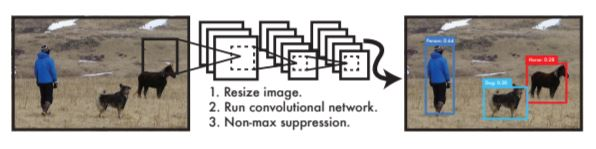
\includegraphics[width=0.7\textwidth]{chapter2/images/yolo.jpg}
    \caption{กระบวนการทำงานของโครงสร้างโมเดลปัญญาประดิษฐ์ของ YOLO}
    \label{fig:yolo}
\end{figure}

โครงสร้างโมเดลปัญญาประดิษฐ์ของ YOLO เป็นโครงสร้างที่มีความเร็วมาก มีความเร็วในการประมวลผลถึง 45 เฟรมต่อวิ ทำให้สามารถประมวลผลแบบเรียลไทม์ได้ นอกจากนั้นยังมีความแม่นยำ mAP มากกว่าโมเดลสำหรับตรวจจับวัตถุอื่นๆถึง 2 เท่า ซึ่งเหตุผลที่โครงสร้างโมเดลปัญญาประดิษฐ์ของ YOLO เร็วกว่าโมเดลปัญญาประดิษฐ์ตัวอื่นๆ เนื่องจาก มีแนวคิดที่ต่างออกไป คือ สำหรับการตรวจจับวัตถุในวิธีการก่อนหน้าจะใช้วิธีทำนายกรอบสี่เหลี่ยมก่อน แล้วจึงค่อยนำกรอบสี่เหลี่ยมไปทำนายว่าเป็นหมวดหมู่อะไร ซึ่ง YOLO มีวิธีการที่ต่างออกไป คือ ทำนายกรอบสี่เหลี่ยมและทำนายว่ากรอบสี่เหลี่ยมนั้นเป็นหมวดหมู่อะไรพร้อมกัน โดยใช้โครงข่ายประสาทแบบคอนโวลูชั่น ด้วยแนวคิดนี้จึงเป็นที่มาของชื่อ YOLO หรือ you only look once การมองแค่เพียงครั้งเดียว ซึ่งโครงสร้างโมเดลปัญญาประดิษฐ์ของ YOLO ที่ถูกใช้ในงานวิจัยนี้ประกอบไปด้วย 1) YOLOv3-tiny 2)YOLOv3 3) YOLOv3-spp	ซึ่งทั้ง 3 โครงสร้างจะมีความแตกต่างของโครงสร้างดังนี้
\begin{enumerate}
	\setlength\itemsep{-0.25em}
	\item YOLOv3-tiny ใช้ Max-Pooling layers ในขั้นตอนของการลดจำนวนข้อมูลตัวอย่าง
	\item YOLOv3 ใช้ Convolutional layers ในขั้นตอนของการลดจำนวนข้อมูลตัวอย่าง
	\item YOLOv3-spp ใช้ Convolutional layers+ฟีเจอร์ที่ดีที่สุดของ Max-Pooling layers ในขั้นตอนของการลดจำนวนข้อมูลตัวอย่าง
\end{enumerate}
%ข้อมูลผลการทำงานของโมเดลปัญญาประดิษฐ์สำหรับการทำการตรวจจับภาพบุคคล อ้างอิงข้อมูลจากเว็บไซต์ของ YOLO
%\begin{table}[!ht]
%	\begin{tabular}{|c|c|c|}
%		\hline
%		{}&{ความเร็วต่อรูปภาพ (มิลลิวินาที)}&{ความแม่นยำ (0.5 IoU mAP)}			\\
%		\hline
%		SSD Mobilenet v1 ppn	 		& 26				& 20														\\
%		YOLO-v3 320				& 22				& 51.5				\\	
%		YOLO-v3 tiny				& 4.5				& 33.1				\\
%		YOLO-v3 spp				& 50				& 60.6				\\	
%		Faster RCNN inceptrion v2		& 58				& 28		\\
%	\hline
%	\end{tabular}
%	\caption{ข้อมูลผลการทำงานของโมเดลปัญญาประดิษฐ์สำหรับการทำการตรวจจับภาพบุคคล อ้างอิงข้อมูลจากเว็บไซต์ของ YOLO}
%\end{table}

